\chapter{Implementation} \label{cha:implementation}
	The Bachelor Project course would not be a real Bachelor Project course if 
	there were projects without technical challenges whatsoever regarding the 
	implementation of the final result. Therefore, this chapter elaborates
	on the technical challenges faced during development of the project and
	the solutions that we have developed for these challenges.
	%TODO Highlight technical challenges and elaborate on solutions for these challenges.
	%     This includes (amongst others) how the AR functionality posed a problem and we
	%     implemented a C++ server using OpenCV to take over that work (along with 
	%     synchronizing on a central camera).
	
	% Sections are purely by example. This list might not be entirely correct or complete.
	\section{AR Glasses} \label{sec:arglasses}
		One of the first design choices that we had to make was about what
		AR glass was going to be used with the project. As can be seen in
		our research report, under appendix \ref{app:researchreport},
		there two options to choose from. These were the Oculus and
		the META One. We eventually settled for the META One, because
		of the latency of the Oculus. A pair of META Glasses can be seen in
		figure \ref{fig:metaone}.
		
		\begin{figure}[!ht]
			\centering
			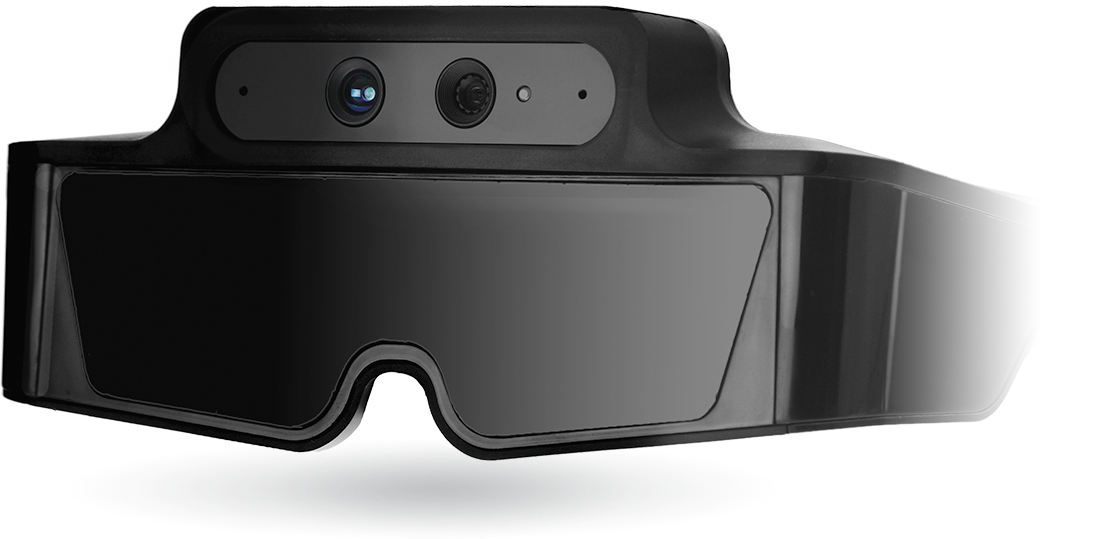
\includegraphics[width=\textwidth]{MetaOneGlasses}
			\caption{A pair of META One glasses.}
			\label{fig:metaone}
		\end{figure}
		
		The challenge with the META One was to get it working in Unity.
		There is a Meta SDK which allows for Unity games to work with
		the META One, but AR itself is still in development (as of
		writing this report), and the META One glasses are experimental
		at best. The SDK that we used first was also very buggy (due to the
		experimental nature of the META One). Also, the META One has a very
		limited field-of-view (the field-of-view was so limited that, during
		one of our first tests with our coach, the coach had to sit back
		to keep everything tracked, which, especially considering that they
		had to move markers as well as track the environment continuously,
		was less than ideal). However, the SLAM tracking built into the
		META allows for game objects to continue to be rendered on a marker
		even if the marker is outside of the view of the META. SLAM tracking
		is explained in subsection \ref{ssec:slamloc}.
		
		\subsection{SLAM tracking} \label{ssec:slamloc}
			SLAM is an acronym, which means Simultaneous Localization And
			Mapping. It stands for a computational problem making a map
			from an unknown environment while updating the location of the
			agent in the same environment. These problems cannot be solved
			independently from each other, as updating a map usually involves
			knowing the location of the agent before any accurate updates
			can be made, and vice versa. Several algorithms have been developed
			for solving this problem, and there is even a platform, called OpenSLAM,
			which contains several open source algorithms which solve this
			problem.
			
			However, the algorithms are beside the point. the real benefit of 
			using SLAM with AR is that SLAM tracking allows the META One to
			render the game objects belonging to a marker while keeping them
			rendered once the marker leaves the field-of-view of the META One.
			Considering that the field-of-view of the META One is not that large
			(As seen in our research report under Appendix \ref{app:researchreport}),
			this is a huge benefit. The META One also has built-in support for
			SLAM tracking of objects, which meant that no time had to be spent
			on developing algorithms.

	\section{Marker Detection} \label{sec:markerdetection}
		...
		
	\section{Synchronization of World State} \label{sec:synchronization}
		Because the game is played by multiple people, the state of the world
        somehow has to be synchronized between all players. To do this, we 
        considered two major options:
        
        The first option was to use the built-in Network View component in 
        Unity. This would allow Unity to take care of most synchronization,
        which in turn could make implementing the synchronization particularly
        easy. However, due to the way the Meta One glasses manipulate the 
        positions and rotations of game objects to fit the orientation of the 
        player's head, synchronizing these positions would result in incorrect
        positions for other players. Instead, a custom serialization method 
        would have to be implemented to undo the manipulation by the Meta One
        and then apply the correct manipulation for each of the other players.
        
        Because of the issues the Network View component would give, a second
        option was considered. This option would introduce the need for a 
        master server that hosted the game, and could provide raw positions
        and rotations of markers exactly as they were placed on the table.
        The only thing left to do would be to move and rotate the objects for 
        each player to match that player's view of the playing area. 
        Additionally, the server approach also solved another recurring issue,
        as highlighted in section \ref{sec:markerdetection}.
        
        In the end, we went for the second option because of the abovementioned
        reasons, but also partly because it allowed us more control over the 
        internal workings of the network functionality and the marker tracking.
        See section \ref{sec:markerdetection} for the details about the marker
        detection performed by the server.
		
	\section{Networking and the OpenCV server} \label{sec:network}
		The game depends on a server application with a master camera. The 
        server application detects the position and rotation of markers in the 
        playing area. It does this through the use of a central so-called master 
        camera, that is position so that the entire playing area is visible from 
        the camera.
        
        The server application is written in C++ and is based on OpenCV and the 
        Qt framework. We decided to implement the server outside of Unity, since 
        Unity does much more than what we need of the server. The server only 
        acts as a way to track all markers even if they aren't seen by any of 
        the players, and to facilitate synchronizing state changes with all 
        players. For example, if a remote player rotates an object in the game, 
        the details about that rotation is sent to the server, which then 
        distributes it to all other players.
        
        A more detailed description about the communication between the Unity 
        clients and the server can be found in paragraph \ref{ssec:communication}.
        The use of the master camera to detect markers is described in paragraph
        \ref{ssec:mastercamera}.
         		
		\subsection{Communication between C\# and C++} \label{ssec:communication}
			Communication between the Unity clients and the OpenCV server 
            happens through the use of sockets. For the Unity side, the Socket 
            facility built into the C\# runtime is used. For the OpenCV server, 
            the TCP Socket facility of the Qt Network module is used for 
            providing a server socket capable of handling multiple clients. 
            
            The protocol used for communication is kept very simple to reduce 
            network load and for simplicity. The protocol consists of a number
            tag indicating the message type followed by the actual message 
            content. To facilitate the features the game provides, the following
            message types are used:
            
            \begin{description}
                \item[Position Update] Sent by the server whenever it detects a 
                                       change in a marker position.
                \item[Position Delete] Sent by the server whenever a marker is
                                       removed from the playing field.
                \item[Rotation Update] Sent by remote players to indicate they 
                                       have rotated an object. This message is 
                                       forwarded to all connected clients by the
                                       server.
                \item[Ping Message]    Sent by the server and clients to indicate 
                                       they are still connected and listening.
            \end{description}
		
		\subsection{The master camera} \label{ssec:mastercamera}
			...
			
	\section{Distinguishable markers} \label{sec:markers}
		...